\subsection{Use Case Models}
User case diagram:\\
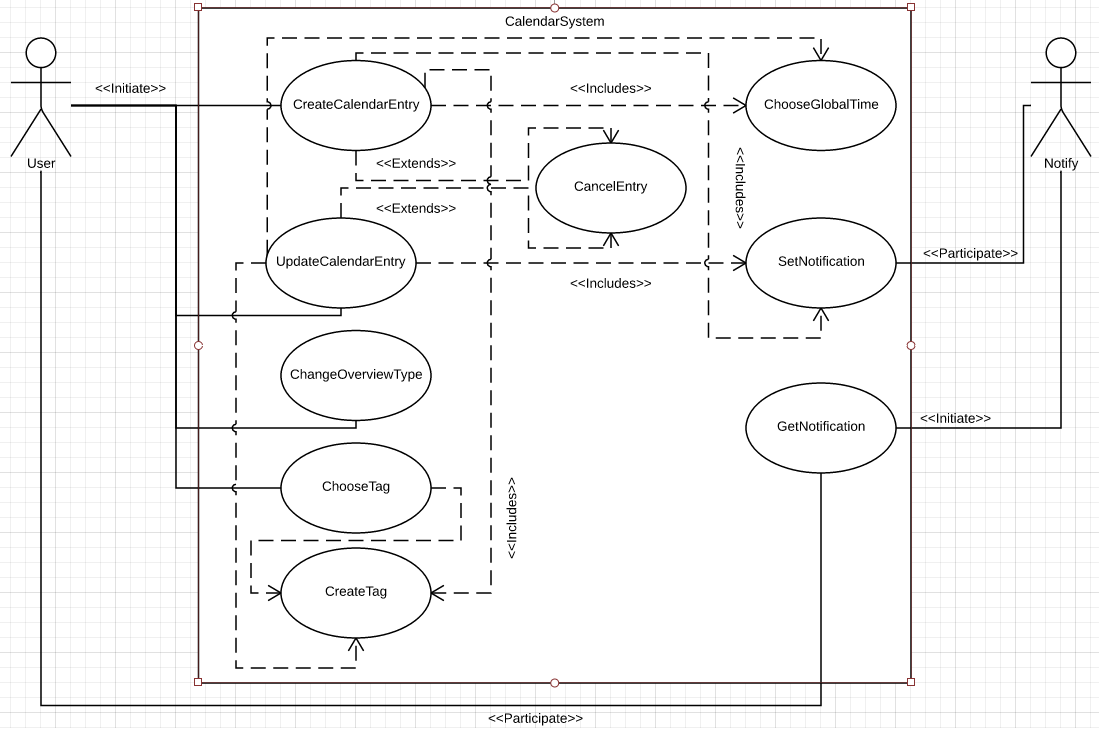
\includegraphics[scale=0.6]{CalendarSystemUseCaseDiagram}\\\\
Here you can see a short description of the three user cases CreateTag, ChooseTag and GetNotifikation\\\\
\textbf{User Case name: CreateTag}\\
\HRule \\[0.4cm]
\textbf{Participating Actors:}\\
Initiated by User\\
Communicates with PAC-CLOUD data storage\\
\HRule \\[0.4cm]
\textbf{Flow of events}\\
User initiates the CreateTag\\
User chooses a name for the tag\\
 - Exceptional case: User cancels the creation.\\
User accepts and finish\\
\HRule \\[0.4cm]
\textbf{Entry Condition}\\
The user has logged into the CALENDARSYSTEM\\
The user is in the tag drop down menu OR creating an Event or Updating an Event\\
\HRule \\[0.4cm]
\textbf{EXIT Condition}\\
The user has created a tag or cancelled the creation\\\\\\
\textbf{User Case name: ChooseTag}\\
\HRule \\[0.4cm]
\textbf{Participating Actors:}\\
Initiated by User\\
Communicates with PAC-CLOUD data storage\\
\HRule \\[0.4cm]
\textbf{Flow of events}\\
User opens the TAG drop down menu\\
 - Exceptional case: CreateTag use case - user wants to create a new tag\\
 - Exceptional case: user closes the dropdown menu\\
User chooses between his tags or <All>\\
The Calendar overview is updated with all events with the tag.\\
\HRule \\[0.4cm]
\textbf{Entry Condition}\\
The user has logged into the CALENDARSYSTEM\\
\HRule \\[0.4cm]
\textbf{EXIT Condition}\\
The user has picked a tag or choosen to keep the current tag\\\\\\
\textbf{User Case name: GetNotifikation}\\
\HRule \\[0.4cm]
\textbf{Participating Actors:}\\
Initiated by CALENDARSYSTEM\\
Communicates with PAC-CLOUD data storage\\
Prompted to the user\\
\HRule \\[0.4cm]
\textbf{Flow of events}\\
CALENDARSYSTEM creates a popup with a notifikation message of the event\\
User reads the notification\\
\HRule \\[0.4cm]
\textbf{Entry Condition}\\
The user has logged into the CALENDARSYSTEM\\
CALENDARSYSTEM has a notifikation from an event set at a specific time.\\
\HRule \\[0.4cm]
\textbf{EXIT Condition}\\
User closes the notification\\

\newpage